\documentclass[../../main.tex]{subfiles}

\begin{document}

Assuming the tree $T$ created above is accurate, we now seek to infer genotypes from this phylogeny so as to overcome errors and noise associated with low coverage SCS data.
We first determine weights for attaching point mutations and different types of LOH events to different edges of the tree, and then use these weights to determine genotype probabilities for each cell.
The approximate phylogeny was found by combing information from across the genome, however to infer cell genotypes we shall return to considering individual loci.

\subsubsection{SNV weights}
In the simplest case, we ignore any potential loss of heterozygosity.
For each edge of the tree $e$, we seek to answer the following question: assuming there is a pont mutation at this locus, what is the probability it occurred at $e$?

To begin with, we compute the probabilities of all descendents of an edge in the tree having the same genotype.
We say that $\pi_0(e), \pi_1(e)$ and $\pi_2(e)$ are respectively the probabilities that all descendents of $e$ are homozygous reference, heterozygous and homozygous alternate.

These values are taken to be
\begin{equation*}
\pi_g(e) = \prod_{\{j:c_j\succ e\}} P(g_j = g)
\end{equation*}
where $c_j\succ e$ indicates that the $j^{th}$ cell is below $e$ in $T$.
$P(g_j = g)$ here are the posterior probabilities calculated in Equation~\eqref{eq:sitebayes}.
We also compute one more value, $\pi_\mu(e)$, defined as the probability that all descendents of $e$ have a genotype of either 1 or 2, that is to say they are mutant.
These four values can be computed recursively in $O(m)$ time by multiplying the corresponding values from the two branches directy beneath each branch.

If an SNV occurred at edge $e$ in $T$, we would expect that all descendents of $e$ would have genotypes of 1 or 2, while all other cells would have genotype 0 (assuming infinite sites).
Letting $\rho$ be the edge ancestral to all sampled cells, it is easy to verify that the likelihood(?) of this simplifies to:
\begin{equation}
    \prod_{c_l\succ e}P(g_l =1,2)\prod_{c_m\nsucc e} P(g_m = 0) = \pi_\mu(e)\frac{\pi_0(\rho)}{\pi_0(e)}
\end{equation}
Since mutations are more likely to occur on longer edges by definition we must (?) scale this value by the prior probability that any mutation occurs on the given branch.
We must undo the Jukes-Cantor correction that was useful for neighbor joining to find a value proportional to the expected number of SNVs along an edge.
We find $\overline{p}_e = \frac{3}{4}\left(1-e^{-\frac{4}{3}d_e}\right)$ to be such a value and therefore define the weight for attaching a SNV to edge $e$ to be:
\begin{equation}
    W(S_e) = \frac{\pi_\mu(e)}{\pi_0(e)} \overline{p}_e
\end{equation}
We have ignored the constant $\pi_0(\rho)$ as it is constant for the locus, and the normalized weights will eventually be used.

\subsubsection*{Weights For Loss of Heterozygosity}
\begin{figure}[h]
	\centering

	\begin{subfigure}{0.2\textwidth}
		\centering
		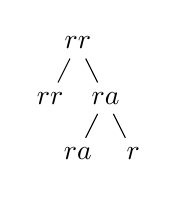
\begin{tikzpicture}[sibling distance=2em, level distance=2em]
  \node {$rr$}
    child { node {$rr$} }
    child { node {$ra$}
      child { node {$ra$} }
      child { node {$r$}}
          };
		\end{tikzpicture}
		\caption{Case 1}
	\end{subfigure}
	\begin{subfigure}{0.2\textwidth}
		\centering
		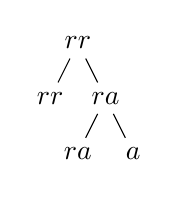
\begin{tikzpicture}[sibling distance=2em, level distance=2em]
  \node {$rr$}
    child { node {$rr$} }
    child { node {$ra$}
      child { node {$ra$} }
      child { node {$a$}}
          };
		\end{tikzpicture}
		\caption{Case 2}
	\end{subfigure}
	\begin{subfigure}{0.2\textwidth}
		\centering
		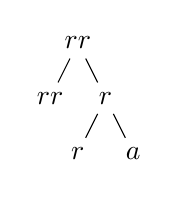
\begin{tikzpicture}[sibling distance=2em, level distance=2em]
  \node {$rr$}
    child { node {$rr$} }
    child { node {$r$}
      child { node {$r$} }
      child { node {$a$}}
          };
		\end{tikzpicture}
		\caption{Case 3}
	\end{subfigure}
	\begin{subfigure}{0.2\textwidth}
		\centering
		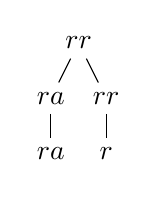
\begin{tikzpicture}[sibling distance=2em, level distance=2em]
  \node {$rr$}
    child { node {$ra$} 
    	child { node {$ra$} }
    	  }
    child { node {$rr$} 
    	child { node {$r$} }
    	};
		\end{tikzpicture}
        \caption{Case 4}
    \end{subfigure}
    \caption{Different ways loss of heterozygosity can occur in a tree.}
    \label{fig:treecases2}
\end{figure}

The more complicated cases invlove both a SNV and a ploidy change occuring at the same locus.
The four possible ways this can occur is shown in Figure~\ref{fig:treecases2}.

Referring to Figure~\ref{fig:treecases2} above these weights are calculated for cases 1, 2 and 3 in the following way:
\begin{equation*}
W^{(1)}(S_{e_1},L_{e_2}) = \frac{\pi_0(e_2)\pi_1(e_1)}{\pi_1(e_2)\pi_0(e_1)}d_{e_1}P(L_{e_2})
\end{equation*}
\begin{equation*}
W^{(2)}(S_{e_1},L_{e_2}) = \frac{\pi_2(e_2)\pi_1(e_1)}{\pi_1(e_2)\pi_0(e_1)}d_{e_1}P(L_{e_2})
\end{equation*}
and
\begin{equation*}
W^{(3)}(S_e) = \frac{\pi_2(e)}{\pi_0(e)}d_e
\end{equation*} 
If a haploid event should occur at the locus under examination, the prior probability that it should occur on edge $e$ is given to be: %TODO may need to lengthen root edge to account for homozygous alternate germline mutations
\begin{equation*}
P(L_e) = \frac{d_e}{\sum_{e'\in E-E_l} d_{e'}}
\end{equation*}
where $E_l$ is the set of all edges directly above leaf nodes. It is assumed that allelic dropout due to amplification is much more frequent than ploidy changes that affect only a single cell, and thus the prior probability of the latter is set to 0. For cases 1 and 2 we define
\begin{equation*}
W'^{(1)}(L_e) = \frac{\sum_{e' \preceq e} W^{(1)}(S_{e'},L_e)}{\sum_{e' \preceq e}W(S_e')} 
\end{equation*}
where the values in the denominator come from Equation~\eqref{eq:Wmu}. Similarly
\begin{equation*}
W'^{(2)}(L_e) = \frac{\sum_{e' \preceq e} W^{(2)}(S_{e'},L_e)}{\sum_{e' \preceq e}W(S_e')} 
\end{equation*}
%TODO this assumes LOH and SNV positions are independent. Is this biased for those highr or lower or neither?
Finally, assuming an SNV has already occured at the given locus, the probability of a case 1 haploid event happening at any edge $e$ is given by (see appendix ??):
\begin{equation*}
P(L_e^{(1)}) = P(L_e^{(1)}\mid S_{\preceq e}) = \frac{P(LOH)}{3} \frac{W'^{(1)}(L_e)}{\sum_{e'\in E-E_l}W'^{(1)}(L_{e'})}
\end{equation*}
and under the same assumption, the conditional probability for case 2:
\begin{equation*}
P(L_e^{(2)}) = P(L_e^{(2)}\mid S_{\preceq e}) = \frac{P(LOH)}{3} \frac{W'^{(2)}(L_e)}{\sum_{e'\in E-E_l}W'^{(2)}(L_{e'})}
\end{equation*}
The probability for case 3 is given by
\begin{equation*}
P(L_e^{(3)}) = P(L_e^{(3)}\mid S_{\preceq e}) = \frac{P(LOH)}{3} \frac{W^{(3)}(L_e)}{\sum_{e'\in E-E_l}W^{(3)}(L_{e'})}
\end{equation*}
The prior probability $P(LOH)$ of a loss of heterozygosity occuring at the site given that a SNV has occured is given to be
\begin{equation*}
P(LOH) = P(LOH_i \mid SNV_i) = \frac{3}{2}\cdot\frac{1-\prod_j\left[P(g_{ij}=0)+P(g_{ij}=1)\right]}{1-P(\sigma_i = 0)}
\end{equation*}

\subsubsection*{Genotyping Cells}
%TODO got to keep a running probability of case 3, separate from genotype probs. prob of 2 from 0 = p(S_e)*(sum(P(case 3 ancestral))+case2 at e)
With all of these values computed for each of the edges in the tree, we can use a dynamic programming algorithm to genotype the cells. We complete a depth first traversal of the tree keeping track of genotype probabilities at every node. We also keep track of the probability $P(L_{\preceq e}^{(3)})$ that a silent case 3 haploid event has occured ancestral to each node. The initial conditions for the root node are the genotype probabilities $P(g=0)=1$ and $P(g=1)=P(g=2)$ and $P(L_{\preceq \rho}^{(3)}) = 0$. Let $n_1$ be the direct ancestor of $n_2$ such that $n_1$ and $n_2$ are joined by $e$ and have genotypes $g_1$ and $g_2$ respectively. Therefore we define the relations:
\begin{equation*}
P(L^{(3)}_{\preceq n_2}) = P(L^{(3)}_{\preceq n_1}) +P(L^{(3)}_e)
\end{equation*}
\begin{align*}
P(g_2 = 0) = &P(g_1=0)\left[(1-P(S_e))+P(S_e)P(L^{(1)}_e)\right]\\
+ &P(g_1 = 1)\left[P(L^{(1)}_e)\right]
\end{align*}
%TODO is it necessary to include that no type 3, is that assumed?
\begin{align*}
P(g_2 = 1) = &P(g_1=0)\left[P(S_e)(1-P(L^{(1)}_e)-P(L^{(2)}_e))\right]\\
+ &P(g_1 = 1)\left[1-P(L^{(1)}_e)-P(L^{(2)}_e)\right]
\end{align*}
%TODO do we need 1-P(S_e) here?
\begin{align*}
P(g_2=2) = &P(g_1=0)\left[P(S_e)(P(L^{(3)}_{\preceq n_2}) + P(L^{(2)}_e))\right]\\
+ &P(g_1=1)\left[P(L^{(2)}_e)\right]\\
+ &P(g_1=2)
\end{align*}

When the tree traversal reaches the leaf nodes, these are taken to be the cell genotype probabilities. The cell will be genotyped in accordance with the highest probability.


\end{document}
